
\section{General Solar System Inertial and Fixed Systems} \label{sec:gen} 
Established here is the generic coordinate system of solar system bodies as set by the International Astronomical Union \cite{IAU2006} and adopted by the PDS.  The IAU system applies to all bodies in the solar system. The IAU defined transformation from inertial to body fixed is given by a simple formulation for all solar system bodies. The general ICRS is a coordinate system with its origin at the solar system body center and axis directions that are defined as parallel to those of the ICRS system. See section \ref{sec:bcrf} for definition of the ICRS and section \ref{sec:gendet} for a more formal relation between inertial and rotating system.

In JEOD more refined and sophisticated body orientation parameters are needed for non-spherical gravitational fields. In particular the transformation from inertial to body fixed exist for the Earth, Moon and Mars, the reader is referred the relevant body orientation system for these bodies, see \hypermodelref{TIME}\  for the Earth and Mars and \hypermodelref{EPHEMERIDES} for the Moon.  For all other bodies such planets, asteroids, satellites and dwarf planets, only the IAU orientation parameters are currently included in JEOD. 

Figure \ref{fig:2} presented here is the IAU cannonical standard or IAU generic fixed coordinate frame. The pole is specified as the two intersection points of the body's equator and the ICRF equator define it as the node Q. The prime meridian has been chosen so that it crosses the body's equator at point B.\\
\begin{itemize}
\item $\alpha_0$ = right ascension of pole.\\
\item $\delta_0$ = declination of the pole.\\
\item $\aries$  is the direction of Ares at epoch J2000.\\
\item W = location of the prime meridian Q with respect to B.\\
\end{itemize}
\textbf{Coordinate Frame: } IAU generic fixed.

\begin{itemize}
\item X-axis: Defined as the cross product of the Z-axis (as defined below) and the Earth mean orbit pole of J2000 (i.e. the ecliptic pole of J2000). The X-axis of this coordinate frame is the
Earth vernal equinox of J2000.
\item Y-axis: Completes a standard, right-handed coordinate frame.
\item Z-axis: Defined as the pole vector of the Earth Mean Equator of J2000
(where J2000 = Julian date 2451545.0).
\end{itemize}


\begin{figure}[htp]
\centering
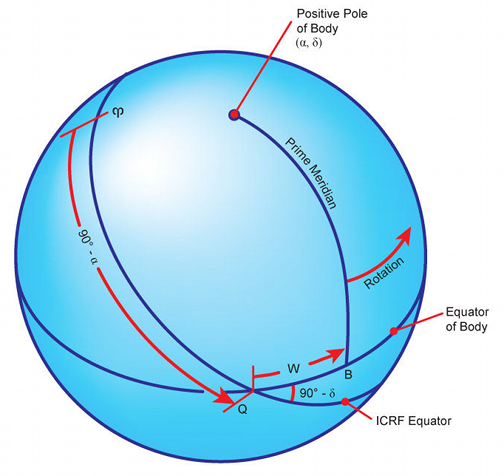
\includegraphics [width=7in]{figs/fig2.png}
\caption{IAU Pole and Meridian Definitions}
\label{fig:2}
\end{figure}

\subsection{Example General IAU Body System}
See section \ref{sec:gendet} for elaboration.



